\subsection{Caso d'uso UC11: Salvataggio di un progetto}
\begin{figure}[h] 
	\centering 
	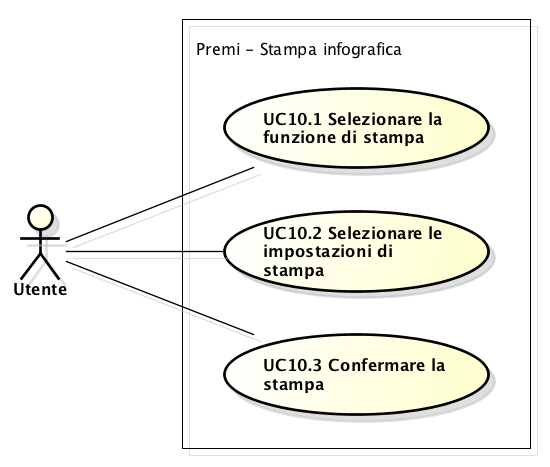
\includegraphics[scale=0.45] {img/UC11.png}
	\caption{UC11 - Salvataggio di un progetto} 
\end{figure}

\begin{itemize}
	\item \textbf{Attori:} Proprietario;
	\item \textbf{Scopo e descrizione:} L'utente ha creato un progetto e vuole salvare il suo stato per poterlo aprire successivamente;
	\item \textbf{Precondizione:} L'utente ha creato un progetto nella fase di creazione;
	\item \textbf{Flusso principale degli eventi:}
	\begin{enumerate}
		\item L'utente seleziona la funzione salva [UC11.1];
		\item L'utente inserisce il nome del progetto [UC11.2];
	\end{enumerate}
	\item \textbf{Postcondizione:} Il sistema ha salvato il progetto nel server con il nome indicato dall'utente.
\end{itemize}


\subsection{Caso d'uso UC11.1: Selezionare la funzione salva}
\begin{itemize}
	\item \textbf{Attori:} Proprietario;
	\item \textbf{Scopo e descrizione:} L'utente seleziona dall'apposito menù la funzione di salvataggio per salvare il progetto;
	\item \textbf{Precondizione:} Il sistema è in attesa che l'utente selezioni la funzione salva;
	\item \textbf{Postcondizione:} Il sistema ha aperto la finestra di dialogo per il salvataggio.
\end{itemize}


\subsection{Caso d'uso UC11.2: Inserire il nome del file}
\begin{itemize}
	\item \textbf{Attori:} Proprietario;
	\item \textbf{Scopo e descrizione:} L'utente deve inserire un nome valido con il quale salvare il progetto;
	\item \textbf{Precondizione:} Il sistema permette all'utente di inserire il nome della presentazione da salvare;
	\item \textbf{Postcondizione:} È stato inserito un nome valido per il progetto e il sistema lo salva nel server.
\end{itemize}

